\section{Implementation}
  This meant that it was going to be ideal associating electronic hardware with
  each component of the kart. This was especially important as to minimise the
  delay for PID control of the actuators meant that a higher baud rate was
  required. 

  \subsection{Schematics}
  Using Altium Designer the schematics were laid out. Two techniques were used
  to minimise mistakes in the PCB design. One was to divide all the schematic
  sections onto separate sheets. The other was to be methodical and make notes
  on the sheets if something was not complete. Part of being methodical also
  meant making sure all components were well labelled, even some with comments
  next to them to help explain their existence. This meant when the schematics
  were printed off and reviewed by the whole team, mistakes could be easily
  spotted.
  
  \begin{figure*}[h]
      \centering
      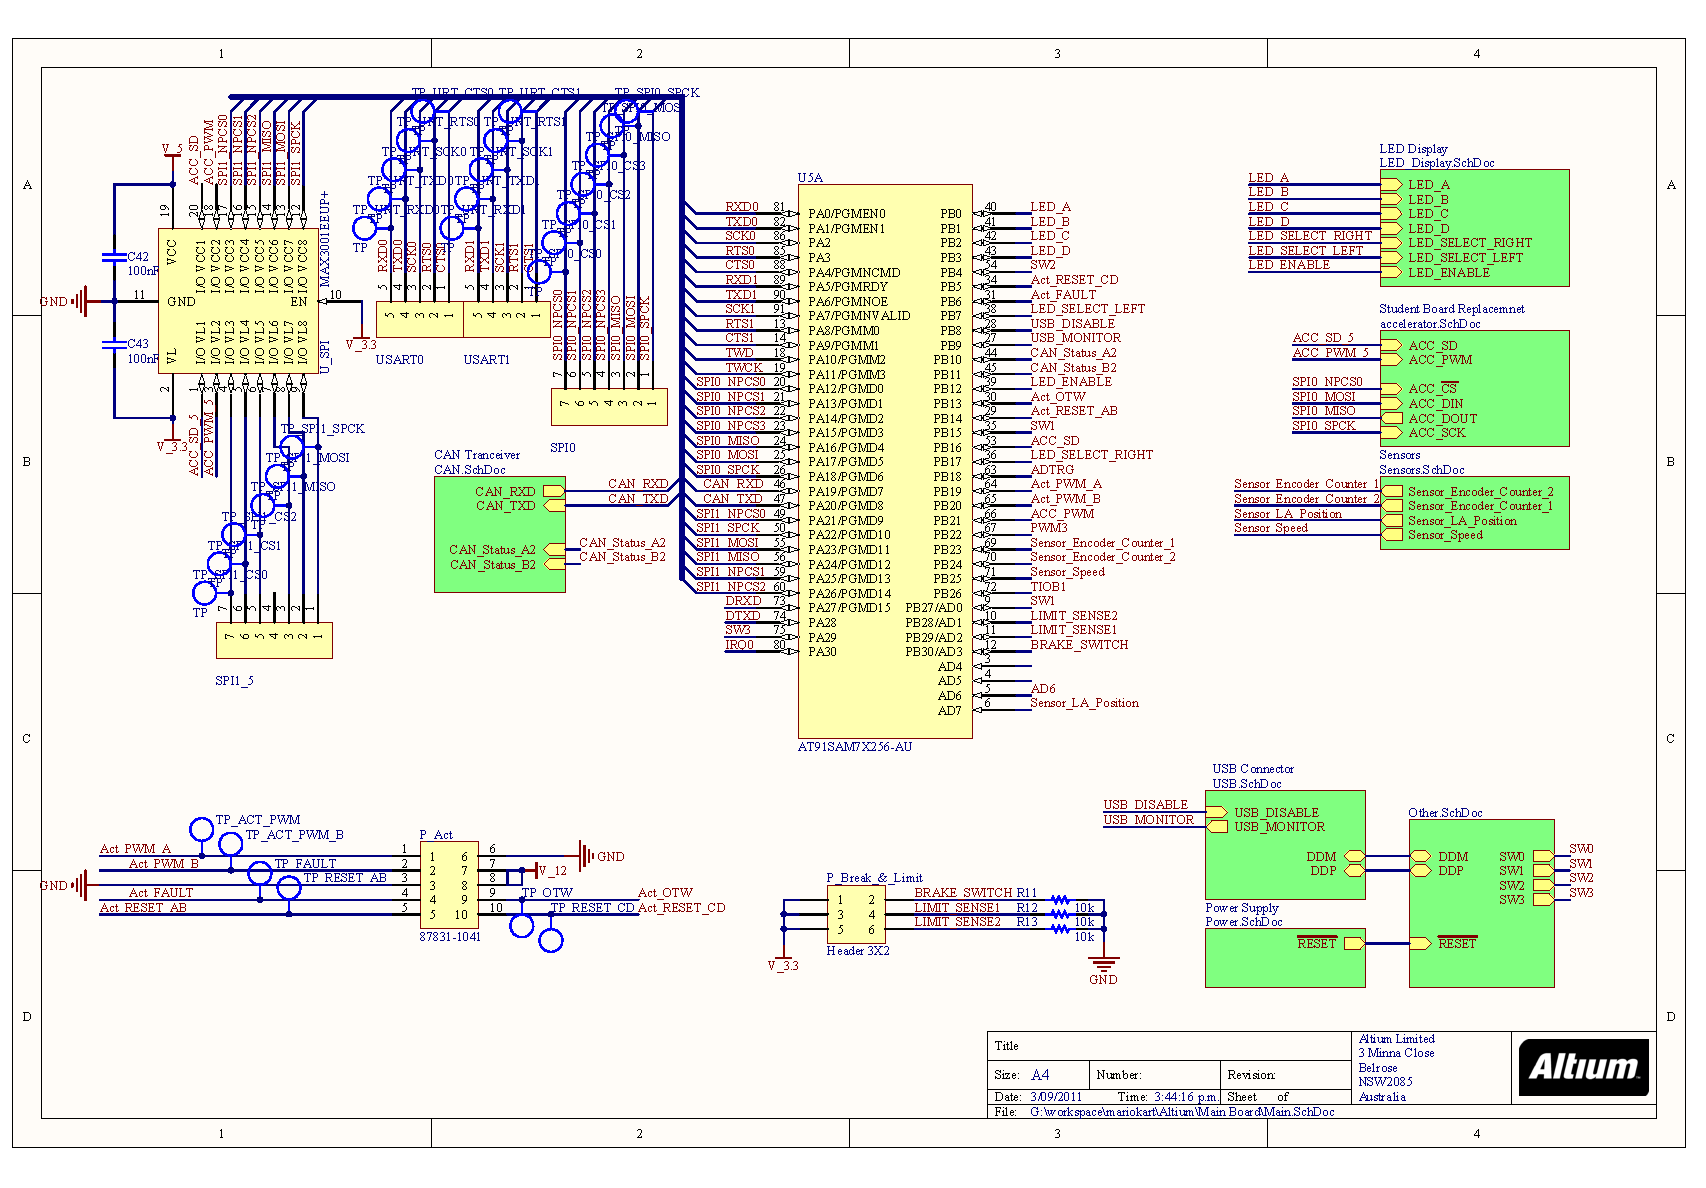
\includegraphics[width=.8\linewidth]{../../Presentation/Henry/Images/Schematic.pdf}
      \caption{Top level schematic for the main PCB.}
      \label{main-schematic}
  \end{figure*}

  Figure \ref{main-schematic} shows the top level schematic with the MCU in the
  middle of the page. The green boxes on the sheet show where other sub sheets
  have been included and wired up. For example, doing this all the decoupling
  capacitors for the micro controller can be essentially hidden in one of these
  sub sheets. 

  \subsection{PCB Design}
  The PCB layout design work was also done in Altium Designer. While the tool
  does not automatically do the layout for the user, it does provides many
  useful tools to aid the process. By setting up the design rules to match the
  manufactures specifications, the manufacture process is sped up eliminating
  them rejecting your design because of design rule violations.

  The main technique that was used when laying out the PCB was to arrange
  clusters of components that are all related. Then place these modules on the
  PCB area. This also allowed the placing of decoupling capacitors in the
  correct locations next to the pin that required the decoupling.
  
  One key rule that was stuck to when laying the PCB was to only put small
  components on the bottom. This allowed the population of the whole bottom side
  of the PCBs then when populating the top side, the components would not fall
  off the bottom in the oven. It also meant we could fit the PCBs in the lid of
  the enclosure that we designed the boards to fit in. The small resistors and
  capacitors don't even touch the inside of the lid.

  \subsection{Components}
  Where possible surface mount technology (SMT) components were selected. This
  has the benefit that it minimises the amount of drilling required to be done
  by the manufacturer. It is also easier to source SMT components. In the final
  design only some connectors are non-SMT.

  \subsection{PCB Manufacture}
  To allow four layer PCBs to be used, the PCBs needed to be manufactured
  off-shore. Because of recommendations by staff in the department, either
  Advanced Circuits in America\cite{advancedCircuits} or OurPCB Tech in
  China\cite{ourPCB} were our best options.  Because of price, Advanced Circuits
  were used. All up for 3 panels, which included all 5 main PCBs and two motor
  driver daughter boards, the charge was 362 USD including shipping. The panels
  were manually cut into the individual PCBs, using a band saw.
  
  \subsection{PCB Population}
  Component population was done by hand initially using a PCB oven, then
  reverting back to hand soldering once the bulk of the components were on the
  PCBs. Population was done in stages, to allow testing of the boards at each
  stage. Figure \ref{fullPCB} shows the brake PCB with all it's components on
  it.
  
  \begin{figure}[h]
      \centering
      \includegraphics[width=.9\linewidth]{../../Presentation/Henry/Images/PCB.png}
      \caption{The populated brake PCB}
      \label{fullPCB}
  \end{figure}

  \subsection{Hardware Testing}
  Before the PCBs even had any components put on them they were tested for
  manufacturing and design flaws. Simply using a multi meter, checking to make
  sure the power planes were not shorted and other key pads were connected as
  they should have been. Then at every stage especially making sure the power
  and ground planes were not shorted was a key concept. At several stages
  shorted pins were picked up because of this testing.

  Once the PCBs had their micro controller placed on its PCB, led test code was
  written to ensure we were able to program and control the board. This also
  helped to pick up shoddy soldering on a couple of the micro controllers. The
  same was repeted for the CAN Bus, push buttons and USB.
